\documentclass[AutoFakeBold]{LZUThesis}

\begin{document}
\title{{关于群众对于社区工作的了解}{和基层社区实际工作情况调查}}


\entitle{{}{}}

\author{许忞欢}
\major{电子信息科学与技术}
\kahao{320200910141}
\advisor{}
\college{信息科学与工程学院}
\grade{2020}



\maketitle
\frontmatter

%中文摘要
\ZhAbstract{中文摘要}{关,键,词}

%生成目录
\tableofcontents
\thispagestyle{empty}


%文章主体
\mainmatter
\chapter{绪 \qquad 论}
作为新时代的大学生,很难说我们这一代人不是在学校里长大的。我们不可以两耳不闻窗外事,要做到既学习专业知识,又了解世界变局。 但与此同时,身边的社会基层工作者常常被我们忽略,而疫情期间基层工作者的重要性再次被体现,而了解基层工作的最好方法就是作为一名大学生更是一名居民去参与,去提出自己的见解,将自己全身心的投入。此外,我还想让更多的人知道更详细的工作细节,这有助于社区的发展,同时锻炼了我自身的能力。

从小学到初中,从高中到大学,我们接触得到的事物无非就是书本上的理论,和老师口传心授的知识。而其中必须要学习的就是我们的思政课,在思政课上我们学会做学生,学会做孩子;到了大学,思政课更加地理论化,教会我们怎样去学习前辈们的思想,怎样理解我们这个世界,我们该用怎样的眼光来看待这个世界是大学里面的老师想要告诉我们的。

归根究底,人类是社会性动物,如果我们光有理论知识是不行的,还要学会和别人打交道。这就让我想起了我国的基层组织,新闻上报道的基层干部们都是积极了解本地情况,在这样的基础上为我国乡村振兴做出巨大贡献。

而作为生活在一个工业小镇上的我来说,社区就是我能想到的最接近的,也是第一时间能够想到的基层组织了。参观学习,跟随,学习社区基层工作,体验基层工作所遇到的困难,作为大学生 给出青年一代的见解和建议,并在能力范围之内参加志愿活动,将自己的学习到的 东西,进一步加深理解与体会。而在本次暑期实践中,我将要前往的是位于江苏省宜兴市官林镇的官林社区,坐落于官林这样一个沿海地区的工业小镇,在七月份,宜兴市全市受疫情影响,即使非中高风险地区,大多数的企业,单位都被要求不出县,不出市。

在这种特殊时期,管控工作也不能放松,这就成为大学生能够参观学习疫情防控的最好时期,中国的疫情防控全世界的人类都有目共睹,所以我一直想要去了解一下疫情防控时期的街道社区的工作究竟应该如何进行。那么,在我的家乡的这样一个小镇里,基层的社区工作人员的具体工作究竟如何,我们作为群众又该如何配合工作呢?

由此,我此行的目的就是

\begin{enumerate}
    \item 调查群众对于社区工作的了解
    \item 了解社区工作人员最近的工作
\end{enumerate}

\chapter{实施调查}

在返家的途中,得到了计划外的收获。七月初,兰州疫情肆虐,打乱了所有人的计划,我临时决定进行返家,这也是导致我势必经过疫情地区。

乘坐高铁到达重点站宜兴站时,第一次体验了落地检。当时是晚上十点左右,受亚热带季风气候影响,天气炎热,在这样的工作环境下,穿着“大白”服装的社区工作人员和志愿者们还坚守在岗位上,进行检查健康码、行程码,询问来访地区和当地住所以及提醒三天两检的工作。

那是我第一次接触到三天两检这样一个名词,而后我在网络上查询到,三天两检是指在3天(72小时)内进行2次核酸检测,两次核酸检测时间需间隔24小时,一般是第一天进行一次核酸检测,第三天进行第二次核酸检测。

因为我当时填错了所在社区,所以第二天到实际所在地区报备后,同时有了两个社区组织通过电话联系我并催促我进行三天两检。这种社区来电一般都有所谓的“闪信”提醒,“闪信”又名“0级短信”,是一种在屏幕上即时显示的、强制接收方阅读的特殊文本信息。当时我对此深感兴趣,查阅资料后知道这是早就有的技术,早在2017年,反诈骗中心就已经通过闪信等方式进行诈骗行为的防治了。

对于这类知识的了解是群众配合工作的基础,为了调查社区工作的情况,关于大众了解这类工作手段的情况和大众对于社区工作的满意度是必要的。

% \begin{figure}[!h]
% 	\centering
% 	\includegraphics[width=6 in]{../pic/voiceOri.png}
% 	\caption{Spectrum of My Voice}
% 	\label{fig:voiceSpectrum}
% \end{figure}

\section{群众调查}

\subsection{基本信息}

在如图\ref{fig:age}所示的调查中,我们可以看到在各个年龄段中都有调查对象进行了我们的调查,其中$35 \sim 40$岁以及$50$岁以上的调查对象较多,这是因为其中参与调查的父辈和祖辈的人数比较多,但是同时年轻群众的参与率也不低,所以结合如图\ref{fig:sex}中所示的调查者的性别而言,我们能看见, 各个年龄段之间以及男女性别之间并不存在很大的误差,所以这次调查拥有其科学性和严谨性。

所以,我会在这个调查报告的接下去的内容中逐步介绍调查的成果,同时结合我的个人层面上的认知,对于这个调查的结果进行尽可能严谨而客观的数据上的分析。

\begin{figure}[!h]
	\centering
	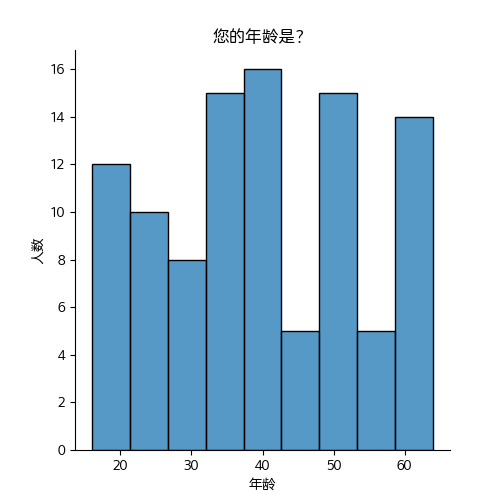
\includegraphics[width=4 in]{figures/age.png}
	\caption{调查者的年龄}
	\label{fig:age}
\end{figure}

\begin{figure}[!h]
	\centering
	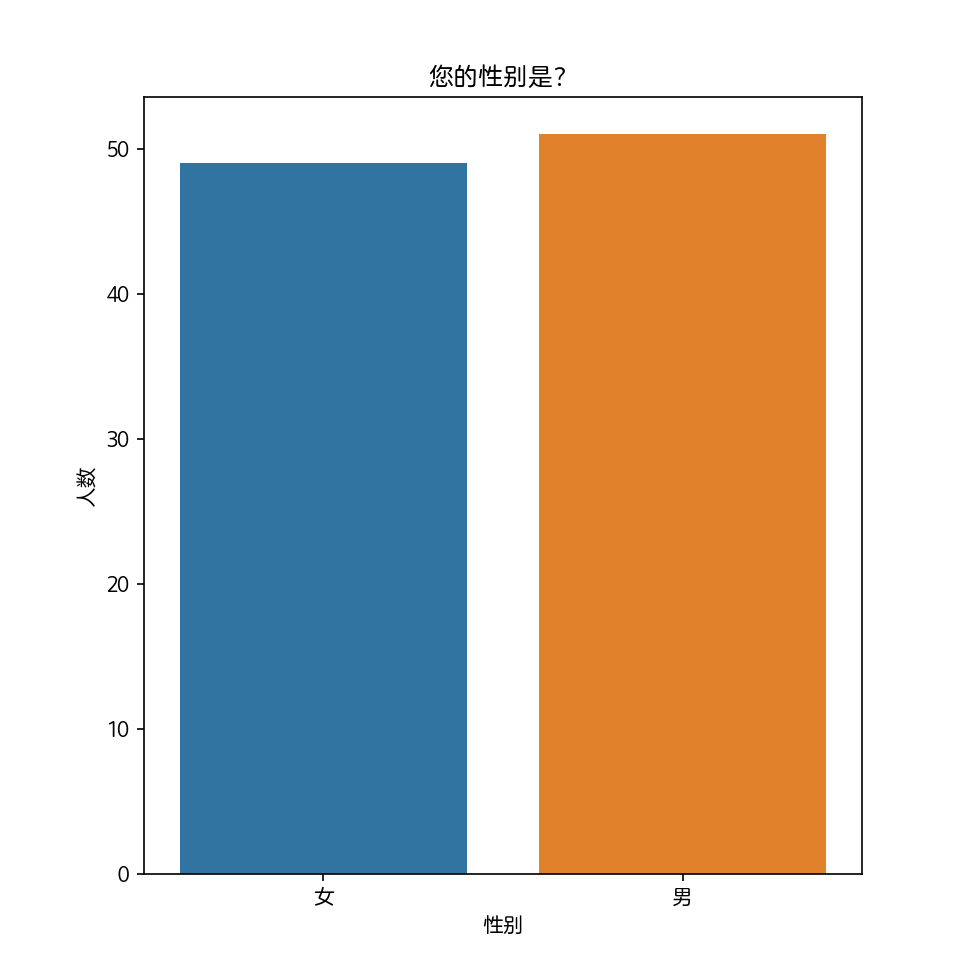
\includegraphics[width=4 in]{figures/sex.png}
	\caption{调查者的性别}
	\label{fig:sex}
\end{figure}

\subsection{所属社区调查}
尽管本次的调查中,以及后续的工作调查都是在宜兴市官林镇官林社区进行的调查工作,但是我们的调查问卷是在整个宜兴市内进行分发填写以及统计的,所以在调查者中会出现三个境内不同的社区,他们分别是官林社区,凌霞社区以及新街社区。这样分发问卷的最终考虑是为了考虑到调查社区工作尽管受限于活动范围而不能进一步扩大,但是我们可以将满意度调查和认知调查延展到邻近的几个社区,以便于更加了解当地普遍的社区工作的情况,并不与我们最初的工作的要求相悖。同时,我们尽可能保证了在官林社区参与调查的人员是最多的,这也是为了在数据上体现我们这次调查的主阵地就是官林社区这样有且仅有的一个社区,尽最大努力保持尽可能保证调查实例化的特征,真正表现最贴切实际的数据在生活上的表现。

\begin{figure}[!h]
	\centering
	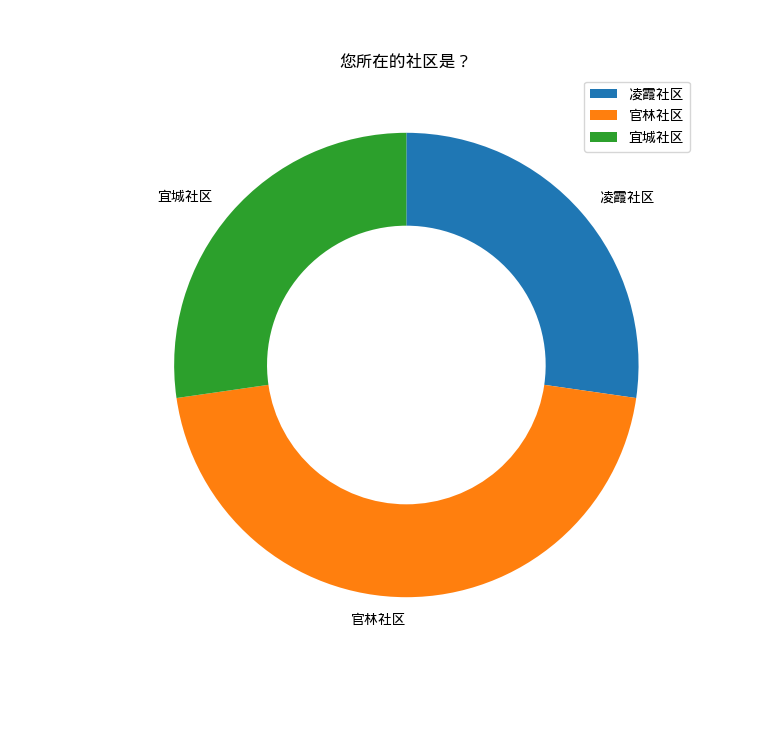
\includegraphics[width=4 in]{figures/community.png}
	\caption{来自不同的社区的调查者}
	\label{fig:community}
\end{figure}

\subsection{社区工作认知调查}
我们可以在如图\ref{fig:lastCom}中得到下面所要阐述的发现,在一天以内以及在一周之内进入过社区的调查者在数量上占很大的优势,约$50\%$以上,占据绝对性优势,这说明群众在支持社区工作,或者配合社区工作以及向社区寻求帮助的人数比较众多。

据了解,由于时值暑假刚刚放假的时期,外来返乡的大学生以及将要返乡的外来务工人员及其子女都需要进行人员流动。其中返乡大学生需要进行三天两检,与此同时,应防疫需求,需要在核酸检测的同时进入社区进行外来地区的报备工作,这也间接导致了调查人员中最近进入社区的人员数量众多。同时,数据中值得注意的是,一年以内和一年以外进入过社区的人员也为数众多,结合实际情况和理论分析后得出,数据中的这部分人是在当地有着稳定的生活,平时没有到社区进行事务办理或者核酸检测等的服务内容的人群。

\begin{figure}[!h]
	\centering
	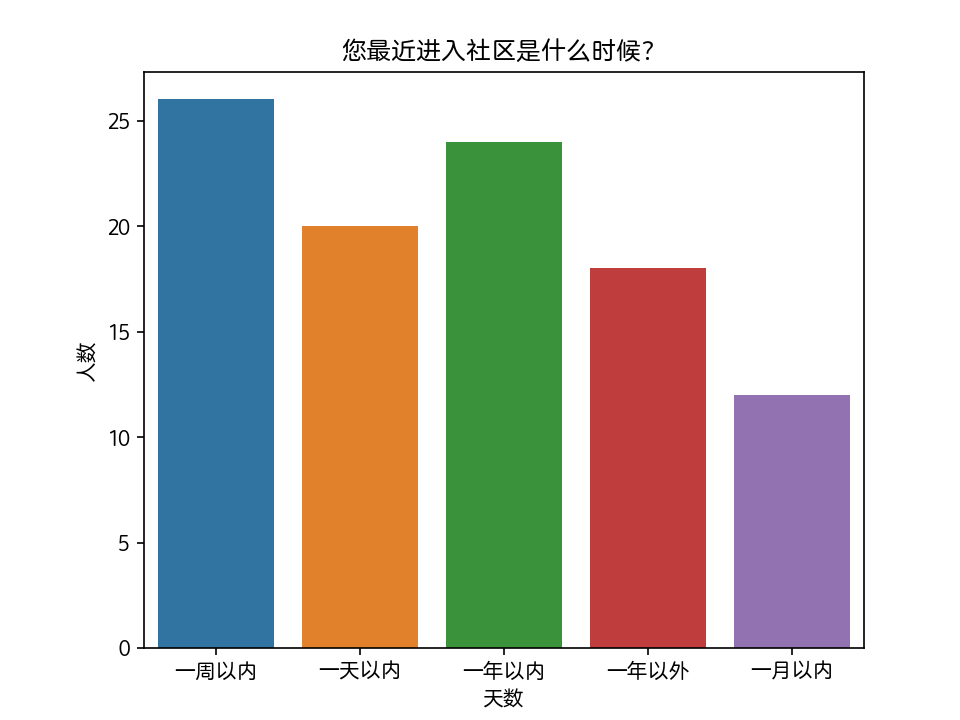
\includegraphics[width=4 in]{figures/lastCom.png}
	\caption{您最近进入社区是什么时候?}
	\label{fig:lastCom}
\end{figure}

这样的情况其实十分有趣,我们结合如图\ref{fig:bother}中所示的调查,其中选项“不知道”和“完全没有”这两个选项占大多数的原因一是社区工作做得十分完善,在做实事的同时,又尽可能做到不打扰群众,这是非常好的,但是令人担忧的是,既然有将近五分之二的调查者最近没有去过社区进行事务办理,他们对于社区工作的评判不一定十分完善,这是在本调查需要改善的不足。

总而言之,我们仍然可以断言,既然受到打扰的群众相较之下比较少,同时没有收到较大的打扰,这是实行工作所必须要面对的一些问题,是所有事情在向好发展的象征。有句话说的好,不怕有问题,就怕没“毛病”,如果调查结果“完全没有”的选项占绝大多数,那证明大多数人都没有社区工作就在身边的感受,同样反映了群众参与程度堪忧的问题。

\begin{figure}[!h]
	\centering
	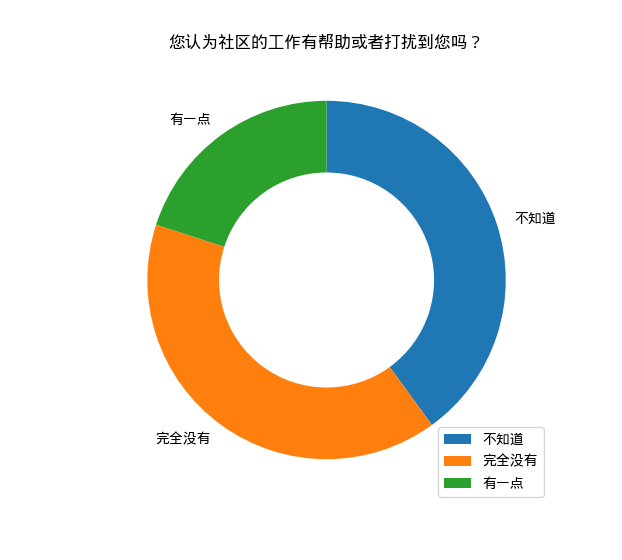
\includegraphics[width=4 in]{figures/bother.png}
	\caption{您认为社区的工作有帮助或者打扰到您吗?}
	\label{fig:bother}
\end{figure}

\subsection{社区知识调查}


% 回到家后,与当地社区协商后决定在项目前期以参观为主,后期进行志愿活动。

% 我第一个参观的工作是江苏省自建房安全排查与鉴定,主要工作为针对自建房的安全问题进行排查。有关项目介绍如下:

% - 排查范围:各地要对本行政区域内城乡所有自建房进行排查摸底,在继续推进农村房屋安全隐患排查整治工作的基础上,重点排查城乡结合部、城中村、安置区、学校医院周边、工业园区等区域,突出人员密集、涉及公共安全的经营性自建房。省级人民政府可根据实际确定具体范围,确保不留死角、不留盲区。
% - 排查内容。各地要全面摸清自建房基本情况,重点排查结构安全性(设计、施工、 使用等情况)、经营安全性(相关经营许可、场所安全要求等落实情况)、房屋建设合法合规性(土地、规划、建设等手续办理情况)等内容。
% 在具体工作中,我了解到本地区绝大多数的自建房屋都是砌体结构,指的就是由块体和砂浆砌筑而成的墙、柱作为房屋主要受力构件的结构的建筑。

% 针对这项工作,相关公司与机构专门出台了一个软件作为工作辅助,在征求工作人员同意后,我对软件的功能进行了探索。平台的名字叫做住房和城乡建设部统一开发信息归集平台,在住房和城乡建设部、 省(自治区、直辖市)住房和城乡建设主管部门两级进行部署, 地市和区县用户通过网络接入访问。值得注意的是,平台计划中由各级承担自建房安全专项整治任务的有关部门保障必要的设施和环境,采取必要的安全措施,确保排查工作的安全有序进行。

% 其最主要的功能是提供实地访查时的卫星地图,在这个地图上有自动(可手工调整)生成的建筑网格,在每个网格中有一个个的建筑,其中同一栋的建筑中可能有不同的所有人,而同一个人可能拥有两栋不同的建筑房屋,而实地考察要做的就是将这个建筑的所有人等基本信息录入系统,并分期对建筑的安全性进行考核,若存在安全隐患则应督促其整改。

% 在跟随社区工作人员和志愿者前往实地考察的时候,发现实地考察的难度远远超过我的想象。

% 1. 首先,根据GPS定位虽然可以实时显示手机所在地址,但是存在不可忽略的延迟,这对于通过并不十分清晰的卫星照片判断影像和房屋实际位置是不小的障碍。
% 2. 其次,今年夏天江苏省迎来了近年来最高温度的暑假,光是站在太阳底下就令人汗如雨下。
% 3. 最后,或是因为家里无人或是老人耳背等原因,导致访查工作迟迟不能进行。

% 为了克服这些困难,社区工作人员多日在同一个地方进行调查,能够做到对某片房屋的门牌及其所有人等信息如数家珍。
% 在实践中,我对于自建房屋工作的数字化程度感到吃惊,完整的录入系统,强大的卫星地图,都有效地帮助了实现物理和社会层面上的双重管理,是数字化办公的典范。但核酸检测的身份录入采用的是拍照的形式,在云端进行文字识别,以达到输入的目的,但是系统仅支持身份证输入,而对于其他能够证明身份的证件(如户口本,台胞证等)并未支持,这是一个值得改进的地方,可能凭借我目前的知识并不能对这样的现状进行改进,但是这是个很好的开始,此次实践教会我的是如何在实际生活中发现问题和关心这些问题,能够在任何方面和层次上对社会做出一点贡献,都是值得的。

\begin{figure}[!h]
	\centering
	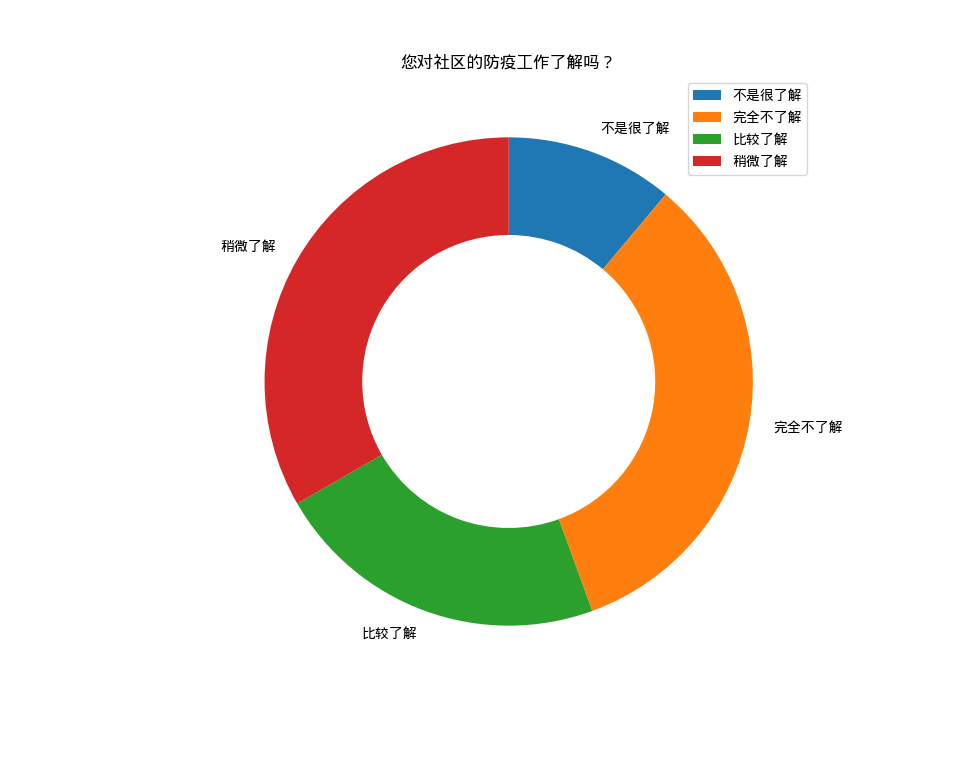
\includegraphics[width=4 in]{figures/knowledge.png}
	\caption{您对社区的防疫工作了解吗?}
	\label{fig:knowledge}
\end{figure}


%论文后部
\backmatter
%引入参考文献文件
\bibdatabase{bib/database}%bib文件名称 仅修改bib/ 后部分
\printbib
% \nocite{*} %显示数据库中有的,但是正文没有引用的文献
\Appendix
\Thanks
\end{document}